\documentclass[conference]{IEEEtran}
\usepackage[T1]{fontenc}
\usepackage[utf8]{inputenc}
\renewcommand{\ttdefault}{lmtt}
\usepackage{amsmath,amssymb,booktabs,array,graphicx}
\usepackage{xcolor,listings,url}
\usepackage[hidelinks]{hyperref}
\hypersetup{pdftitle={EDSO: Connecting Energy Data Governance to AI Evaluation Evidence},pdfauthor={Mohammed Al-Rawi}}
\urlstyle{same}
\newcommand{\term}[1]{\texttt{#1}}
\newcommand{\yes}{Yes}
\newcommand{\no}{No}
\lstset{basicstyle=\ttfamily\scriptsize,breaklines=true,columns=fullflexible,keepspaces=true,frame=single,aboveskip=6pt,belowskip=6pt}
\title{EDSO: Connecting Energy Data Governance to AI Evaluation Evidence}
\author{\IEEEauthorblockN{Mohammed Al-Rawi}
\IEEEauthorblockA{Instituto de Telecomunica\c{c}\~oes\\Aveiro, Portugal}}
\begin{document}
\maketitle
\begin{abstract}
Energy data spaces can expose datasets and services without exposing enough evidence to assess how a model was trained, whether evaluation results are comparable, or which outputs depend on a policy under review. This paper presents the Energy Data Space Ontology (EDSO), a lightweight integration vocabulary connecting local data-use decisions, federated training provenance, scoped privacy statements, model releases, and evaluation evidence. EDSO reuses established vocabularies and provides executable competency questions and SHACL constraints. We investigate its use as an evidence interface for agents selecting energy models. A reproducible experiment on a public, pinned draft executes seven competency queries, seven evaluation-context mutations, four provenance ablations, and five candidate-selection cases. Each context mutation prevents an inappropriate score pairing. One provenance ablation nevertheless passes the current SHACL profile while removing all training-lineage answers, demonstrating why application-specific evidence obligations must complement shape conformance. A small selection gate combines these obligations and rejects the incomplete case. The resulting integration pattern supports evidence retrieval and dependency review across data and AI lifecycles. Proposed applications include energy-community forecasting, municipal building services, and electric-vehicle flexibility. All results concern synthetic metadata fixtures; operational effectiveness remains to be evaluated.
\end{abstract}
\begin{IEEEkeywords}
energy data spaces, ontology, provenance, semantic validation, AI evaluation, agentic AI
\end{IEEEkeywords}

\section{Introduction}
An energy-service agent may discover a forecasting model and its reported error, yet lack the information needed to decide whether that evidence supports its intended task. The error could refer to a different holdout, operating scenario, or model release. A model may also depend on training data governed by a policy that is being revised. These are relationships across artifacts and activities, rather than problems solved by normalizing meter values alone.

Consider an agent assisting an energy community with model selection. Before recommending a model, it should retrieve the relevant evaluation records, identify the contributing sites and data versions, and expose the recorded use decisions. If a policy is subsequently reviewed, the community should be able to find the affected model and its evaluation evidence. Discovery, traceability, and evidence assessment are useful even when a human makes the final decision.

The Energy Data Space Ontology (EDSO)\footnote{Public repository: \url{https://github.com/ITUAV/edso}.} addresses this integration problem through a compact RDF vocabulary, a validation profile, and SPARQL queries. Its starting point is federated energy-model development, but the evidence relationships are also relevant to agents that discover, assess, and recommend AI services. EDSO does not currently represent a complete agent execution lifecycle. It supplies part of the metadata such a lifecycle would consume.

This paper makes three contributions. First, it describes a public integration pattern linking governed data use to model and evaluation evidence, with explicit reuse boundaries. Second, it defines a small, task-specific evidence gate that combines validation, evaluation-context matching, and expected training-site coverage. Third, it evaluates these mechanisms through controlled graph mutations, including a counterexample where shape conformance does not provide the trace completeness needed by the task. The contribution concerns the operational use of metadata; it does not introduce a learning algorithm, a policy-enforcement mechanism, or a safety guarantee.

\section{Related Work and Positioning}
Energy semantics and energy data spaces already have substantial ontology support. SAREF4ENER provides energy-domain concepts for interoperable systems~\cite{saref}. The OMEGA-X Energy Data Set Ontology describes technical and exchange context, including properties, schedules, quality, and participants~\cite{omegax}. Its evaluation point denotes a physical or virtual component associated with exchanged data, rather than an AI evaluation execution. These vocabularies provide complementary domain and data-exchange descriptions.

Janev \emph{et al.}~\cite{janev} investigate semantic technologies for responsible knowledge management in energy data ecosystems, establishing connections among energy data, governance, and analytics. The Intelligent Energy Systems Ontology (IESO) supports communication among agent-based energy systems, applications, and services, drawing on existing energy ontologies~\cite{ieso}. These contributions motivate a more specific research question: how can an energy application check and explain the evidence dependencies of a selected model?

At the cross-domain level, PROV-O represents entities, activities, agents, and their provenance relationships~\cite{prov}; ODRL provides a policy-expression model~\cite{odrl}; and SHACL provides graph-validation machinery~\cite{shacl}. The Data Quality Vocabulary (DQV) supplies reusable quality-measurement patterns~\cite{dqv}. MLDCAT-AP describes machine-learning models, datasets, and associated metadata, including evaluation-related concepts~\cite{mldcat}. EDSO reuses its \term{MachineLearningModel} class rather than asserting that model metadata is absent from existing European specifications.

Public infrastructure initiatives also connect energy data spaces, AI services, and testing facilities. EnerTEF explicitly targets a federated energy AI testing architecture with scenarios, protocols, and metrics~\cite{enertef}. EDSO's intended distinction is consequently narrow: a compact, executable application profile joining data-use decisions and federated provenance to evaluation-context checks and policy-dependency queries. Table~\ref{tab:position} identifies the integration questions addressed here. It is a positioning summary, not an exhaustive feature audit or proof that other vocabularies cannot express the same information.

\begin{table}[t]
\caption{Reuse boundaries and the integration questions in EDSO}
\label{tab:position}
\centering\small
\begin{tabular}{@{}p{0.28\columnwidth}p{0.65\columnwidth}@{}}
\toprule
Existing basis & EDSO application question \\
\midrule
Energy vocabularies & Which versioned energy-data inputs contributed to this evaluated release? \\
DCAT / MLDCAT-AP & How do catalogued data, services, and models connect to executed activities? \\
PROV-O / ODRL & Which recorded use decision and policy version accompany each local contribution? \\
DQV / evaluation metadata & Which scores have matching declared contexts, and which quality evidence concerns synthetic inputs? \\
SHACL & Does profile conformance also supply the trace required by this particular task? \\
\bottomrule
\end{tabular}
\end{table}

\section{Ontology and Executable Profile}
\subsection{Scope and competency questions}
The evaluated draft contains nine EDSO classes, 17 object properties, and six datatype properties. It is an integration vocabulary rather than a replacement for asset, grid, market, or telemetry ontologies. Its RDF artifacts distinguish ontology semantics, instance data, validation constraints, and application queries. This separation permits a consumer to impose additional evidence requirements without changing the meaning of the core classes.

Seven executable competency questions organize the implementation:
\begin{enumerate}
\item Which local inputs, sites, decisions, and policies contributed to a release evaluated at a testing facility?
\item Which gym and facility scores share the declared evaluation context, and what is their difference?
\item What scoped privacy bound and optional ceiling are reported for a training round?
\item Which synthetic evaluation input has a source and a linked quality measurement?
\item Which evidence items and reviewer are associated with a deployment review?
\item Which catalogued service serves a dataset with a stated semantic profile and policy?
\item Which releases and evaluation records depend on a policy version under review?
\end{enumerate}
The final question makes a recorded policy dependency actionable for review. It does not establish that a policy change invalidates all downstream artifacts or requires model deletion.

\subsection{Core entities and links}
Table~\ref{tab:classes} summarizes the classes, and Fig.~\ref{fig:trace} shows the central evidence path. A \term{LocalContribution} identifies an executed local training activity, its input snapshot, execution site, and decision record. An update artifact is generated by that contribution. A \term{FederatedTrainingRound} consumes updates and generates a checkpoint; a model release is derived from that checkpoint. Standard PROV relationships carry these links. Keeping updates and checkpoints as entities distinguishes the artifacts from the activities producing them.

\begin{figure*}[t]
\centering
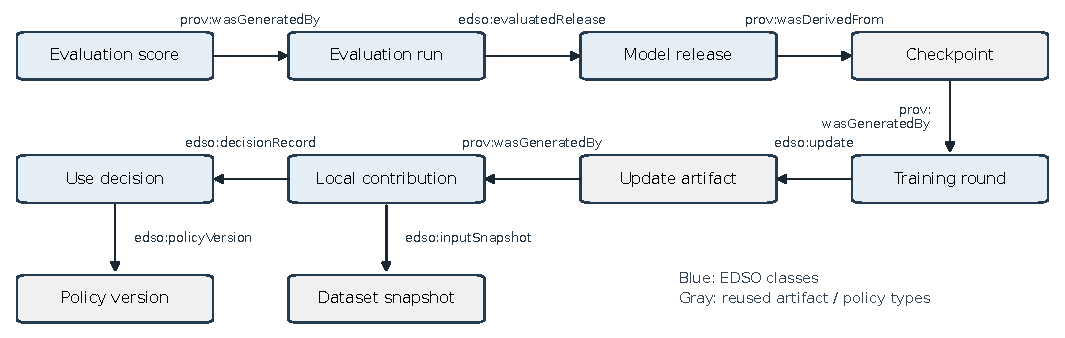
\includegraphics[width=0.98\textwidth]{evidence_path.pdf}
\caption{A central EDSO evidence path. Arrows follow RDF subject--predicate--object direction; they do not depict execution order. Intermediate derivations may occur between a release and checkpoint. Protocol, holdout, scenario, and baseline attach to the evaluation run; metric and unit attach to its score. Checkpoint provenance is required by the lineage query but is not enforced by the tested shape profile.}
\label{fig:trace}
\end{figure*}

\begin{table}[t]
\caption{The nine EDSO classes and their principal reuse}
\label{tab:classes}
\centering\scriptsize
\begin{tabular}{@{}p{0.44\columnwidth}p{0.49\columnwidth}@{}}
\toprule
EDSO class & External superclass(es) \\
\midrule
LocalContribution & prov:Activity \\
FederatedTrainingRound & prov:Activity \\
FoundationModelRelease & ml:MachineLearningModel, prov:Entity \\
UseDecision & prov:Entity \\
PrivacyAccount & prov:Entity \\
SyntheticEnergyDataset & dcat:Dataset, prov:Entity \\
EvaluationRun & prov:Activity \\
EvaluationScore & prov:Entity \\
EvidenceBundle & prov:Collection \\
\bottomrule
\end{tabular}
\end{table}

A \term{UseDecision} records a requested action, requesting agent, dataset, policy version, outcome, and time. The responsible authority is identified with \term{prov:wasAttributedTo}, separately from \term{edso:requestedBy}. A permit record is evidence of a recorded decision; its presence does not authenticate the issuer or replace a policy decision point. The validation profile checks selected relationships, including that the referenced input agrees with the decision's dataset and that the decision precedes the local contribution.

An \term{EvaluationRun} identifies the model release, protocol, holdout, scenario, baseline, execution site, and setting. A score uses \term{prov:wasGeneratedBy} for the run, \term{dct:type} for the metric, \term{rdf:value} for the result, and \term{attr:unitMeasure} for the unit. These external predicates are explicitly documented in the ontology. They avoid competing local definitions of a numeric value or unit.

For a \term{SyntheticEnergyDataset}, source lineage uses \term{prov:wasDerivedFrom}. Dataset quality is represented separately with \term{dqv:hasQualityMeasurement}, \term{dqv:computedOn}, \term{dqv:isMeasurementOf}, and \term{dqv:value}. A fidelity measurement is not evidence of privacy protection. An \term{EvidenceBundle} collects documents and scores using \term{prov:hadMember}, with document types such as bias-audit or impact-assessment records. Such classifications describe evidence, not certified compliance.

\subsection{Privacy statements and validation choices}
A \term{PrivacyAccount} records a reported differential-privacy bound together with its population, protected unit, neighboring-dataset relation, accountant, and scope. An epsilon ceiling is meaningful only for the same stated context; EDSO does not compute privacy composition. Delta accepts decimal or double literals in the validation profile, allowing scientific-notation values produced by typical Python serializers. Range and finite-value checks remain necessary.

Usage annotations identify each property's intended subjects through \term{schema:domainIncludes}, without introducing RDFS domain inferences that could disguise missing instance types. The verification harness supplies the local class hierarchy but disables general inference and remote imports. Lightweight external entity declarations support standalone processing; they are not complete imports of the referenced vocabularies. The draft namespace is tied to the public Turtle location. A stable persistent namespace and a documented migration policy are needed before a long-term identifier commitment.

\section{Task-Specific Evidence Obligations}
\subsection{Conformance is a scoped statement}
Let $G$ be the supplied instance graph, $S$ the fixed SHACL profile, and $C_S(G)$ its conformance result. Conformance states that the supplied graph satisfies the tested constraints at their targets. It is not a completeness assertion about all relevant real-world activities. A consumer must specify the evidence required for its own task and the graph boundary within which absence is treated as missing evidence.

For a model $m$, let $L_G(m)$ be the lineage rows returned by competency query~1, each containing a site, input, decision, and policy. Let $F_m$ be an independently supplied expected set of training sites. A limited coverage requirement is
\begin{equation}
 T(G,m,F_m) = [\pi_{\mathrm{site}}L_G(m)=F_m].
\label{eq:trace}
\end{equation}
Here $F_m$ must come from a trusted training manifest or an explicit test specification, not from the observed rows themselves. Otherwise a missing contributor could redefine the expectation and escape detection. Site coverage remains weaker than complete contribution coverage: two missing jobs at a represented site may be invisible to this test. A production manifest should therefore enumerate expected activities and artifacts as well as sites.

\subsection{Evaluation-context matching}
For a score $s$, define its declared comparison key as
\begin{equation}
 \kappa(s)=(m,p,h,c,b,\mu,u),
\label{eq:key}
\end{equation}
where the components identify model release, protocol, holdout, scenario, baseline, metric, and unit. Query~2 pairs gym and testing-facility scores only when these identifiers agree. It then returns the numeric difference. Matching is deliberately conservative: equivalent units or protocols expressed with different identifiers are not automatically reconciled.

Equality of this key is a metadata precondition, not evidence of statistical equivalence or experimental replication. Hardware, random seeds, runtime dependencies, uncertainty estimates, and temporal distribution shift may matter even when the key matches. Identifier equality also presupposes reliable versioning; a protocol IRI that silently changes content undermines the check. Site and setting are intentionally allowed to differ because the query compares evidence across environments.

\subsection{A candidate-selection gate}
For the fixed request used in the experiment, let $P_G(m)$ denote a nonempty set of matched gym--facility score pairs for $m$. A candidate gate is
\begin{equation}
 A(G,m,F_m)=C_S(G)\land[P_G(m)\ne\varnothing]\land T(G,m,F_m).
\label{eq:gate}
\end{equation}
The first component checks the supplied graph globally; the remaining components concern the target release. This is a small metadata gate, not a general authorization or deployment-admissibility rule. It has no application accuracy threshold and no live operating-state constraints. Its implementation is transparent:
\begin{lstlisting}
valid = validate_profile(graph)
pairs = matching_scores(graph, release)
sites = traced_sites(graph, release)
candidate = valid and bool(pairs) \
            and sites == expected_sites
\end{lstlisting}
An agent can call this deterministic tool and return the supporting records or the missing-evidence reasons to a reviewer. There is no requirement for a language model to infer RDF paths or decide whether an absent record is acceptable.

Policy review is a separate traversal. Query~7 starts from a named policy version, follows the decisions and local contributions that cite it, and returns reachable releases and evaluations. The resulting set is a review worklist. Unrecorded dependencies are outside its reach, and no causal influence or legal consequence follows from reachability alone.

\section{Reproducible Evaluation}
\subsection{Artifact and experimental protocol}
We freeze the public draft at commit
\begin{center}\scriptsize\texttt{0917407b3d343775fd955ba25ae1974d9073cdd7}.\end{center}
The ontology contains 283 triples. The two supplied example graphs contain 190 triples in union, including a federated forecasting illustration and a separate SAREF-based flexibility fragment. The forecasting illustration contains two contributing sites, one round and checkpoint, one release, and gym and facility evaluations. All names and measured values are fixtures. No energy model, controller, or language-model agent is executed in this experiment.

The accompanying \term{evaluate.py} uses RDFLib~7.1.4 and pySHACL~0.30.1. It first runs the existing verification suite: seven expected competency-query results, 15 negative SHACL cases, two query counterexamples, and a Python-float serialization round trip. It then creates a fresh graph copy for every mutation or ablation. This prevents one fault from contaminating the next test. The script records machine-readable outcomes in \term{results.json} and asserts the reported behavior. These are deterministic software checks; no statistical significance or runtime scalability claim is made.

\subsection{Context mutations}
The unmodified fixture returns one matched pair. Its illustrative MAE values are 4.2 and 4.6~kW, yielding a 0.4~kW difference. We independently replace each of the seven key components in Eq.~\eqref{eq:key} on the facility side: release, protocol, holdout, scenario, baseline, metric, and unit. Every mutation reduces the number of matched pairs from one to zero. This verifies that the implemented join uses each declared component. It does not establish that the chosen components are sufficient for every energy application.

\subsection{Provenance ablations}
Table~\ref{tab:ablations} reports four single-edge deletions. The complete fixture has two lineage rows and two policy-impact rows for the policy under review. Removing one local decision or update-provenance link loses the affected contribution. Removing checkpoint provenance or release derivation breaks the common path to both contributors.

\begin{table}[t]
\caption{Single-edge ablations on the metadata fixture}
\label{tab:ablations}
\centering\small
\begin{tabular}{@{}p{0.43\columnwidth}ccc@{}}
\toprule
Removed link & Conforms & Lineage & Impact \\
\midrule
None (reference) & Yes & 2 & 2 \\
Contribution--decision & No & 1 & 0 \\
Update--contribution & No & 1 & 0 \\
Checkpoint--round & Yes & 0 & 0 \\
Release--checkpoint & No & 0 & 0 \\
\bottomrule
\end{tabular}
\vspace{2pt}
\parbox{\columnwidth}{\footnotesize Lineage and impact are query-result row counts, not completeness percentages. Impact is evaluated for the fixture's policy A.}
\end{table}

The checkpoint--round deletion is particularly informative. The graph still conforms to the current SHACL profile, yet no complete release-to-contributor trace is returned. Thus, $C_S(G)$ alone does not imply Eq.~\eqref{eq:trace}. This is a limitation of the tested profile for the stated task, not a limitation inherent to SHACL: a stronger task profile could require this path. EDSO's modular approach allows either stronger shapes or explicit consumer checks. The experiment retains the original profile to expose the difference reproducibly.

\subsection{Candidate gate and interpretation}
The gate uses the two expected fixture sites and the target release. Table~\ref{tab:gate} shows five cases. Conformance alone accepts the altered scenario and missing checkpoint provenance, while the combined gate rejects both. Conversely, its acceptance of the complete fixture only means that the declared metadata obligations have been met.

\begin{table}[t]
\caption{Candidate selection for one declared model request}
\label{tab:gate}
\centering\small
\begin{tabular}{@{}p{0.54\columnwidth}cc@{}}
\toprule
Fixture variant & Conforms & Candidate \\
\midrule
Complete & Yes & Yes \\
Different facility scenario & Yes & No \\
Denied local contribution & No & No \\
Missing score unit & No & No \\
Missing checkpoint provenance & Yes & No \\
\bottomrule
\end{tabular}
\end{table}

These tests establish traceable behavior for a small graph and intentionally selected faults. They do not measure false-acceptance rates on independently curated data, resistance to fabricated metadata, cross-organization semantic agreement, or operational benefit. Mutation tests partly mirror the specified query contract and cannot demonstrate superiority over other ontology stacks. In particular, the underlying vocabularies can express these facts; EDSO supplies a repeatable integration contract and checks. A stronger evaluation should include independent exporters, additional training topologies, policy revisions, and a comparison against a conventional catalog-plus-provenance implementation performing the same tasks.

\section{Applications and Research Agenda}
\subsection{Evidence tools for energy agents}
Here an agent is software that selects and invokes tools to pursue a task, potentially using a language model. Three proposed applications motivate extending the tested integration pattern.

\emph{Energy-community forecasting:} an assistant could retrieve candidate releases, compare their declared evaluation contexts, and produce a recommendation with data-use and training provenance. A changed policy could trigger a review of dependent models and recommendations. The current vocabulary covers the path up to models and evaluation evidence; recording actual recommendations, recipients, and their dependencies requires an application extension.

\emph{Municipal building services:} an agent coordinating multiple public buildings could request evidence that a forecasting or optimization service was evaluated under the relevant climate, occupancy, and demand scenario. Explicit identifiers can prevent scores from unrelated settings being silently pooled. Building semantics, sensor quality, comfort constraints, access control, and online monitoring must be supplied by aligned domain vocabularies and operational systems. No building-control behavior is demonstrated here.

\emph{Electric-vehicle flexibility:} a scheduling assistant could combine SAREF4ENER descriptions with evidence about a model used to estimate flexibility. An evidence record might explain why a forecast was selected, while a separate controller enforces network limits and charging commitments. EDSO's current flexibility example illustrates domain-vocabulary reuse; it is not an implementation of that scheduling workflow.

\subsection{Extensions that should remain explicit}
Broadening the vocabulary should follow demonstrated requirements rather than adding application labels. First, the current \term{FoundationModelRelease} class is too specific for arbitrary forecasting, optimization, and rule-based services. A future profile should introduce or reuse a general model-release concept, retaining foundation-model releases as a specialization and providing a migration path.

Second, a decision-to-action trace would need tool invocations, input-state snapshots, selected services, recommendations, human approval where applicable, executed actions, and observed outcomes. Much of this can reuse PROV entities and activities; new EDSO terms should be introduced only where an explicit competency question cannot be met through documented reuse. A policy review could then reach recommendations and executions, rather than stopping at model evaluations.

Third, evidence validity needs temporal and trust semantics. A useful extension would distinguish creation time, validity period, supersession, issuer identity, and verification status. Metadata provenance alone cannot establish the truth of a reported score or permission. Finally, deployment selection would require performance thresholds, uncertainty, robustness evidence, and application-specific constraints. The gate in Eq.~\eqref{eq:gate} is a starting point for such work, not an adequate production admission procedure.

\subsection{Community development and next evaluation}
The public repository invites competency questions, vocabulary mappings, metadata exports, failing examples, and validation rules through issues and pull requests. Versioned profiles should retain minimal examples and expected query answers to make contributions testable.

A next evaluation should involve at least two independent metadata producers implementing the same profile without coordinating predicate choices informally. Their exports could be tested for query-answer agreement, integration effort, and detection of seeded lineage or context faults. A simulated municipal or community workflow could then compare agents using ordinary catalog descriptions with agents using structured evidence tools. Measures should include unsupported recommendations, missed dependencies, correct abstention, and reviewer effort. Energy or cost savings require a separate controlled operational evaluation; they cannot be inferred from successful metadata validation.

\section{Conclusion}
EDSO connects governed local energy-data use with federated training and evaluation evidence through a small, reusable vocabulary and executable profile. Its value extends beyond data formatting when consumers use these links to check evaluation context and identify policy-dependent artifacts. Controlled experiments show both the intended query behavior and a concrete gap between profile conformance and task-specific trace coverage. Combining those checks offers a practical starting point for evidence-aware energy agents. The public draft and reproducible tests support community development, while independent implementations and application-level evaluation remain necessary to establish broader utility.

\begin{thebibliography}{10}
\bibitem{saref} ETSI, ``SAREF for Energy Flexibility,'' ver. 2.1.1, Jun. 2025. [Online]. Available: \url{https://saref.etsi.org/saref4ener/v2.1.1/}.
\bibitem{omegax} OMEGA-X, ``Energy Data Set Ontology,'' ver. 1.0, 2024. [Online]. Available: \url{https://fz-hannou.github.io/Omega-X/EnergyDataSetOntology.html}.
\bibitem{janev} V. Janev \emph{et al.}, ``Responsible knowledge management in energy data ecosystems,'' \emph{Energies}, vol. 15, no. 11, Art. no. 3973, 2022, doi: 10.3390/en15113973.
\bibitem{ieso} G. Santos, ``Intelligent Energy Systems Ontology,'' ver. 1.1.0, Apr. 2025. [Online]. Available: \url{https://www.gecad.isep.ipp.pt/ieso/v1.1.0/}.
\bibitem{prov} W3C, ``PROV-O: The PROV ontology,'' W3C Recommendation, Apr. 2013. [Online]. Available: \url{https://www.w3.org/TR/prov-o/}.
\bibitem{odrl} W3C, ``ODRL information model 2.2,'' W3C Recommendation, Feb. 2018. [Online]. Available: \url{https://www.w3.org/TR/odrl-model/}.
\bibitem{shacl} W3C, ``Shapes Constraint Language (SHACL),'' W3C Recommendation, Jul. 2017. [Online]. Available: \url{https://www.w3.org/TR/shacl/}.
\bibitem{dqv} W3C, ``Data on the Web best practices: Data Quality Vocabulary,'' W3C Working Group Note, Dec. 2016. [Online]. Available: \url{https://www.w3.org/TR/vocab-dqv/}.
\bibitem{mldcat} European Commission, SEMIC, ``MLDCAT-AP,'' ver. 3.1.0, Candidate Recommendation, May 2026. [Online]. Available: \url{https://semiceu.github.io/MLDCAT-AP/releases/3.1.0/}.
\bibitem{enertef} EnerTEF, ``Project objectives.'' [Online]. Available: \url{https://www.enertef.eu/objectives}. Accessed: Nov. 24, 2026.
\end{thebibliography}
\end{document}
